

              
%Plantilla basada en "Template for Masters / Doctoral Thesis" (plantilla disponible en writeLaTex) que subió LaTeXTemplates.com

\documentclass[11pt]{book}
\usepackage[paperwidth=17cm, paperheight=22.5cm, bottom=2.5cm, right=2.5cm]{geometry}
\usepackage{amssymb,amsmath,amsthm} %paquete para símbolo matemáticos
\usepackage[spanish]{babel}
\usepackage[utf8]{inputenc} %Paquete para escribir acentos y otros símbolos directamente
\usepackage{enumerate}
\usepackage{graphicx}
\usepackage{algorithm}
%\usepackage{subfig} %para poner subfiguras
\graphicspath{{Img/}} %En qué carpeta están las imágenes
\usepackage[nottoc]{tocbibind}
\usepackage[pdftex,
            pdfauthor={NOMBRE DEL AUTOR},
            pdftitle={TÍTULO DE LA TESIS},
            pdfsubject={ÁREA DE LA TESIS},
            pdfkeywords={PALABRAS CLAVE},
            pdfproducer={Latex con hyperref},
            pdfcreator={pdflatex}]{hyperref}



\begin{document}

%----------------------------------------------------------------------------------------
%   COMANDOS PERSONALIZADOS
%----------------------------------------------------------------------------------------

%SI TU TESIS TIENE TEOREMAS Y DEMOSTRACIONES, PUEDES DESCOMENTAR Y USAR LOS SIGUIENTES COMANDOS

%\renewcommand{\proofname}{Demostración}
%\providecommand{\norm}[1]{\lVert#1\rVert} %Provee el comando para producir una norma.
%\providecommand{\innp}[1]{\langle#1\rangle} 
%\newcommand{\seno}{\mathrm{sen}}
%\newcommand{\diff}{\mathrm{d}}

%\newtheorem{teo}{Teorema}[section] 
%\newtheorem{cor}[teo]{Corolario}
%\newtheorem{lem}[teo]{Lema}

%\theoremstyle{definition}
%\newtheorem{dfn}[teo]{Definición}

%\theoremstyle{remark}
%\newtheorem{obs}[teo]{Observación}

%\allowdisplaybreaks


%----------------------------------------------------------------------------------------
%   PORTADA
%----------------------------------------------------------------------------------------

\title{Tesis} %Con este nombre se guardará el proyecto en writeLaTex

\begin{titlepage}
\begin{center}

\textsc{\Large Instituto Tecnológico Autónomo de México}\\[4em]

%Figura
\begin{center}
\includegraphics[height=3cm]{C:/Users/David/Desktop/DocumentosLaTex/itam}
\end{center}

\vspace{4em}

\textsc{\huge \textbf{Mezclas de distribución en esperanza-varianza}}\\[4em]

\textsc{\large Tesis}\\[1em]

\textsc{que para obtener el título}\\[1em]

\textsc{Licenciado en Actuaría}\\[1em]

\textsc{presenta}\\[1em]

\textsc{\Large David Edgardo Castillo Rodríguez}\\[1em]

\textsc{\large Asesor: Juan Carlos Martínez Ovando}

\end{center}

\vspace*{\fill}
\textsc{México, D.F. \hspace*{\fill} 2016}

\end{titlepage}


%----------------------------------------------------------------------------------------
%   DECLARACIÓN
%----------------------------------------------------------------------------------------

\thispagestyle{empty}
\vspace*{\fill}
\begingroup
``Con fundamento en los artículos 21 y 27 de la Ley Federal del Derecho de Autor y como titular de los derechos moral y patrimonial de la obra titulada ``\textbf{TÍTULO DE LA TESIS}'', otorgo de manera gratuita y permanente al Instituto Tecnológico Autónomo de México y a la Biblioteca Raúl Bailléres Jr., la autorización para que fijen la obra en cualquier medio, incluido el electrónico, y la divulguen entre sus usuarios, profesores, estudiantes o terceras personas, sin que pueda percibir por tal divulgación una contraprestación''.

\centering

\hspace{3em}

\textsc{AUTOR}

\vspace{5em}

\rule[1em]{20em}{0.5pt} % Línea para la fecha

\textsc{Fecha}
 
\vspace{8em}

\rule[1em]{20em}{0.5pt} % Línea para la firma

\textsc{Firma}

\endgroup
\vspace*{\fill}


%----------------------------------------------------------------------------------------
%   DEDICATORIA
%----------------------------------------------------------------------------------------

\pagestyle{empty}
\frontmatter

\chapter*{}
\begin{flushright}
\textit{DEDICATORIA}
\end{flushright}


%----------------------------------------------------------------------------------------
%   AGRADECIMIENTOS
%----------------------------------------------------------------------------------------

\chapter*{Agradecimientos}
%\markboth{AGRADECIMIENTOS23}{AGRADECIMIENTOS} % encabezado 

¡Muchas gracias a todos!


%----------------------------------------------------------------------------------------
%   PREFACIO
%----------------------------------------------------------------------------------------

%\chapter*{Prefacio}

%\pagestyle{plain}
%\markboth{PREFACIO23}{PREFACIO} % encabezado 

%PUEDEN QUITAR ESTA PARTE


%----------------------------------------------------------------------------------------
%   TABLA DE CONTENIDOS
%---------------------------------------------------------------------------------------

%\tableofcontents
\chapter*{Capítulos}
	
	1. Introducción\\
	2. Modelo de mezcla en media\\
	2.1. Modelo de mezcla en varianza\\
	2.3. Modelo de mezcla en media-varianza\\
	3. Inferencia estadística\\
	3.1. Noción de distribución tipo mezcla\\
	3.2. Verosimilitud\\
	3.3. Verosimilitud aumentada\\
	3.4. Estimación de parámetros\\
	3.5. Algoritmo\\
	4. Caso de estudio\\
	4.1. Contexto\\
	4.2. Fuentes de información y datos\\
	4.3. Estimación\\
	4.4. Implicaciones\\
	5. Conclusiones y trabajo futuro\\
	

%----------------------------------------------------------------------------------------
%   TESIS
%----------------------------------------------------------------------------------------
\mainmatter %empieza la numeración de las páginas
\pagestyle{headings}

\chapter*{Introducción} 
\chapter*{Modelo de mezcla en media}
Se dice que un vector aleatorio $X$, de dimención p, es una mezcla en media, si dado $u$ se distribuye normal con vector de  medias $u\mu$, y matriz de varianza-covarianza $\Sigma$. La variable aleatoria $u$ está definida en $R_{+}$. Entonces la probabilidad de que X pertenezca a algún subconjunto $S_{p}\in R^{p}$ es:

\begin{equation*}
  P((X_{1},...,X_{p})\in S_{p})=\underset{0}{\overset{\infty }{\int }}N_{p}(X \in S_{p} |u\mu,\Sigma)f_{u}(u)du 
\end{equation*}


 donde  $\mu \in R^{p}$, $\Sigma \in M_{pxp}$ y u es la variable de mezcla.\\

Si nos enfocamos en la distribución marginal de $X$ dado $u$ podemos notar que el valor de $u$ influye en dónde está centrada la distribución, pues ahora el vector de medias pertenece al segmento dirigido $L(\mu)=( u\mu | u\in R_{+}, \mu\in R^{p})$, por lo que si consideramos que $u$ ha tomado el valor de $u_{i}$, y una muestra aleatoria de $X$ dado $u_{i}$, entonces esta muestra estará centrada sobre el segmento dirigido $L(\mu)$ en el punto $u_{i}\mu$, por lo que para valores de $u$ cercanos a uno, la muestra permanece centrada al rededor de $\mu$, mientras que para valores grandes de u, la muestra se aleja en dirección del vector de medias $\mu$. \\


En la siguiente figura se obserba un ejemplo de una distribución tipo mezcla en media con vectro de medias $\mu=(9,11)$ , matriz de varianza-covarianza $\Sigma=(5,.1,.1,4)$, con variable de mezcla distribuida exponencialmente.\\

\begin{figure*}[!]
\centering
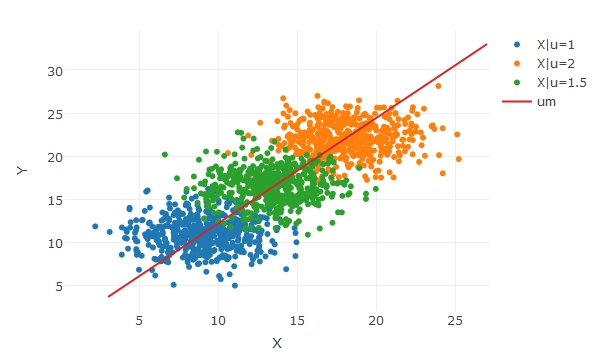
\includegraphics[width=0.7\linewidth]{Rplot}
\caption{Seasumió que u tomó los valores 1, 1.5 y 2.}
\end{figure*}

\pagebreak
\begin{figure}[!]
\centering
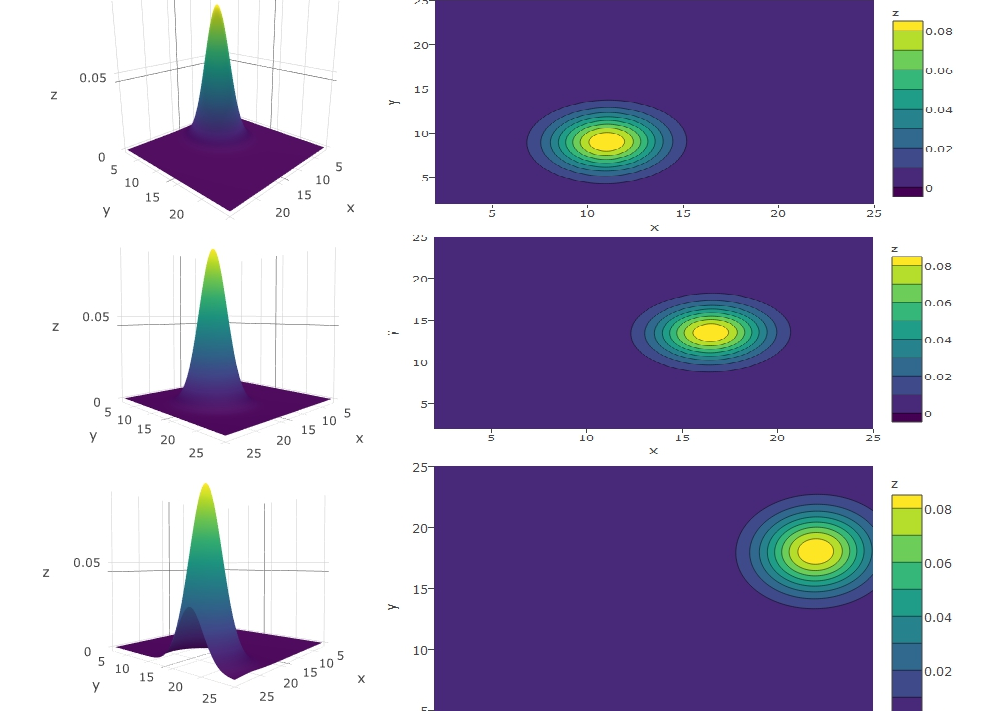
\includegraphics[width=0.7\linewidth]{../mm}
\caption{}
\label{fig:mm}
\end{figure}

En la figura 2 se observa cómo se ve afectada por la variable de mezcla $u$, tanto la función de densidad de $X$ dado $u$, como los contornos del vector aleatorio del ejemplo anterior.\\
\pagebreak

Ahora, si nos enfocamos en la distribución de $X$, tenemos que: 
\begin{equation*}
E[X]=\int_{0}^{\infty}(\int_{D_{X}}XN_{p}(X|u\mu,\Sigma)f_{u}(u)du)dx=
\end{equation*}
Luego, por el teorema de Fubinni:
\begin{equation*}
\int_{0}^{\infty}f_{u}(u)(\int_{D_{X}}XN_{p}(X|u\mu,\Sigma)f_{u}(u)dx)du=\int_{0}^{\infty}f_{u}(u)E[X|u]du
\end{equation*}
\begin{equation*}
\int_{0}^{\infty}f_{u}(u)u\mu du=\mu\int_{0}^{\infty}f_{u}(u)du=\mu E[u]
\end{equation*}
 mientras que $Cov(X)=E[Cov(X|u)]+Cov[E[X|u]]=E[\Sigma]+Cov[u\mu]=\Sigma + var(u)\mu \mu\acute{}$ por el teorema de varianza iterada. Siempre y cuando el segundo momento de $X$ y $u$ existan. Así, la variable de mezcla influye en la localización y disperción del vector aleatorio $X$. Este tipo de mezcla nos permite modelar conjuntos de datos que sigan alguna tendencia con una disperción constante, como se ilustra en la gráfica 1. Por otra parte , una de las mayores difícultades es que,salvo en algunas excepciones, no siempre existe una forma cerrada para la densidad de $X$, por lo que tendría que ser aproximada mediante algún método númerico.\\

Mediante un proceso de simulación se generaron las siguientes gráficas. La gráfica a) proviene de una variable de mezcla exponencial con parámetro $\lambda=1.5$, la gráfica b) proviene de una variable de mezcla gamma con parámetros $\alpha=20$, $\beta=5$, la gráfica c) provine de una variable de mezcla pareto con parámetros $\theta=5$, $\alpha=2$, la gráfica d) proviene de una variable de mezcla Ji-cuadrada con 20 grados de libertad.\\

\begin{figure}[h]
\centering
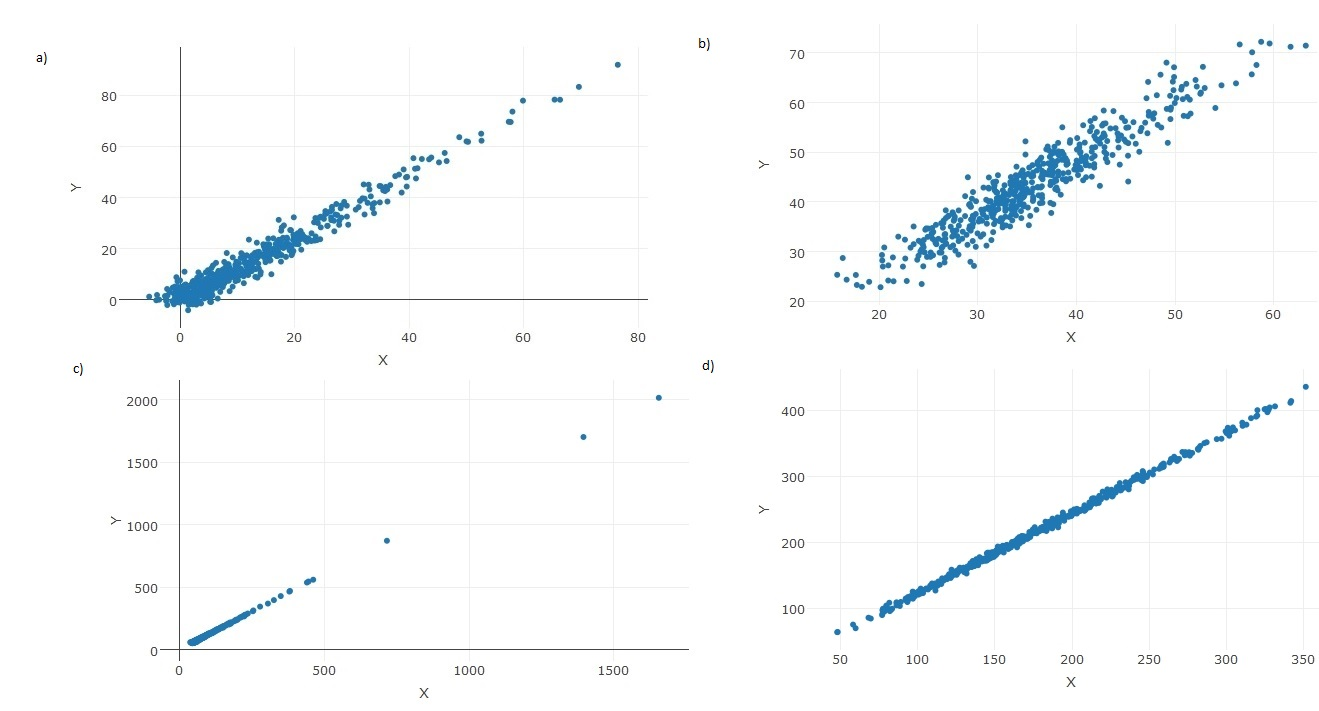
\includegraphics[width=0.7\linewidth]{expo}
\end{figure}


\pagebreak
\subsection*{Modelo de mezcla en varianza}
Ahora considerando un modelo similar al anterior, pero con la diferencia que la variable de mezcla u sólamente afecta a la matriz de varianza-covarianza $\Sigma$, por lo que la distribución del vector aleatorio $X$ p-dimensional viene dado por:

\begin{equation}
P((X_{1},...,X_{p})\in S_{p})=\underset{0}{\overset{\infty }{\int }}N_{p}(X\in S_{p}|\mu,u\Sigma)f_{u}(u)du 
\end{equation}

Si nos concentramos en la distribución condicional de $X$ dado $u$, podemos notar que $u$ influye en la disperción de $X$, por lo que entre mayor sea el valor que tome u, mayor será la disperción al rededor del vector de medias $\mu$, lo cual se ilustra en la siguiente figura. 

\begin{figure}[h]
\centering
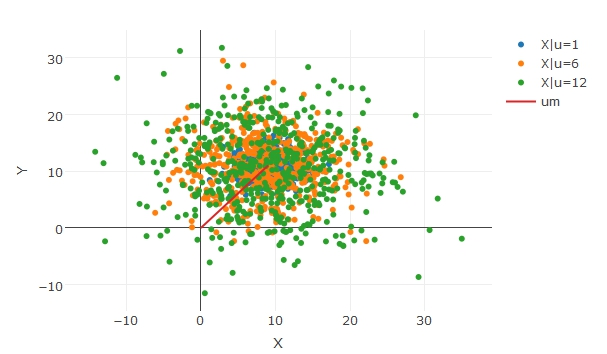
\includegraphics[width=0.7\linewidth]{gvcarregida}
\caption{Se consideraron los mismos parámetros que en la mezcla en media, a excepción de que $u$ tomó los valores 1, 6 y 12 .}
\end{figure}

En la siguiente figura se observa como se modifica tanto la densidad como los contornos de la densidad de $X$ dado $u$, donde $u$ tomó los valores del ejemplo anterior.\\

\pagebreak

\begin{figure}
\centering
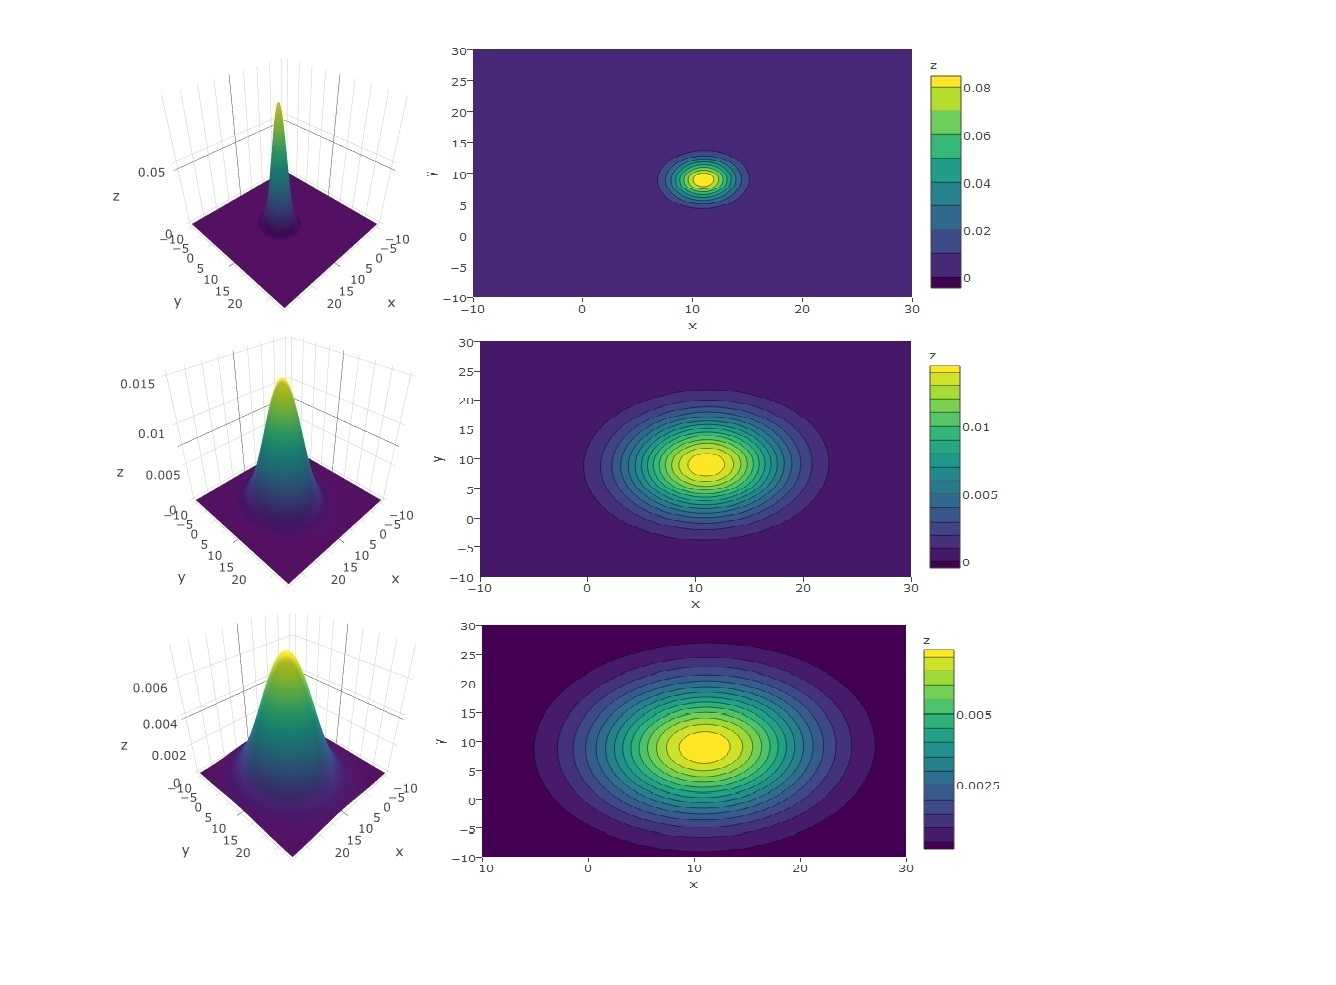
\includegraphics[width=0.7\linewidth]{sv1}
\end{figure}

Ahora considerando la distribución de $X$, es fácil probar que $E[X]=\mu$, y que $Cov[X]=E[u]\Sigma$, por lo que la distribución de $X$ estará centrada en el mismo vector de medias que $X$ dado $u$, mientras que la matriz de covarianzas será proporcional a la matriz de varianza covarianza de $X$ dado u.\\

Ahora se ilustrará, mediante muestras aleatorias, que efecto tiene el condicionamiento en u de la distribución de $X$, adviértase que a diferencia del condicionamiento en media, los datos solo se concentran alrededor del vector de medias $\mu$, pues $E[X]=E[X|u]$, perdiendo la trayectoria del vector de medias, por lo que intuitivamente podemos pensar que $u\mu$ del modelo de mezcla en media generá un vector de trayectoria para las observaciones de $X$.\\

\begin{figure}[h]
\centering
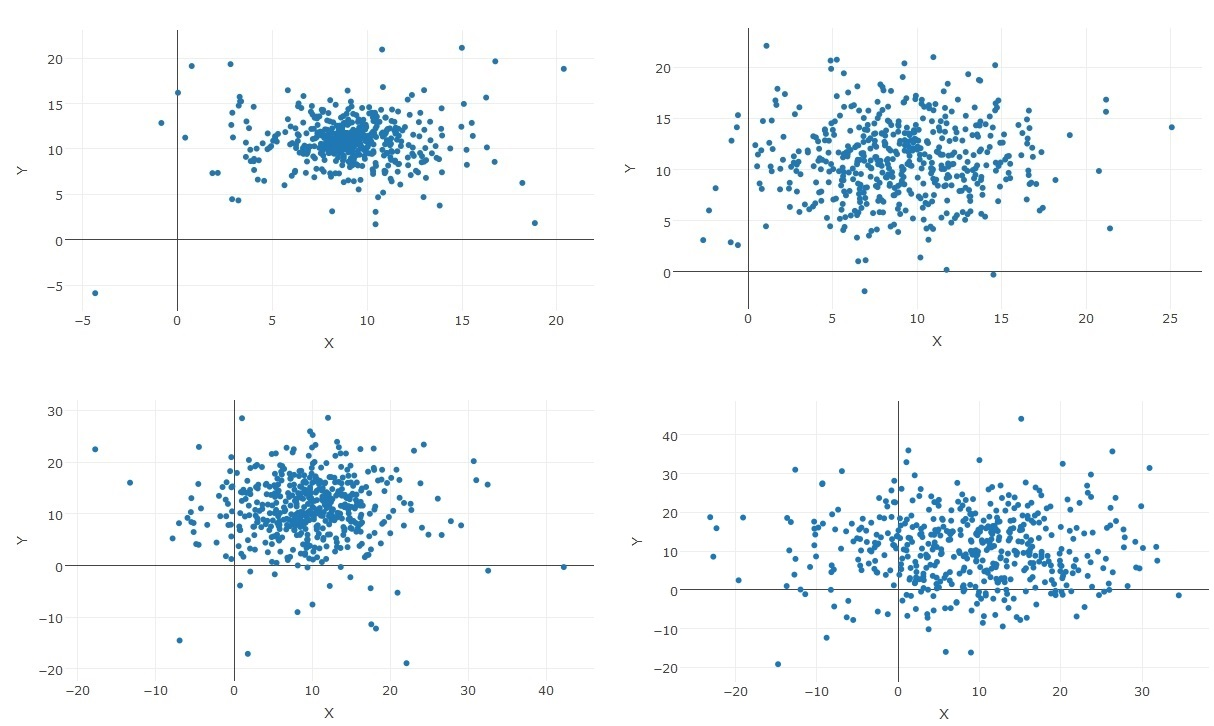
\includegraphics[width=0.7\linewidth]{varianzaexp}
\caption{Se tomaron las mismas distribuciones y parámetros que las gráficas de mezcla en esperanza, pero ahora la variable de mezcla solamente afectó a la matriz de varianza-covarianza.}
\end{figure}


\pagebreak
\subsection*{Modelo de mezcla en esperanza-varianza}

Generalizando los dos modelos anteriores se tiene la siguiente definicion:\\

Se dice que un vector aleatorio $X\in R^{p}$ es un vector tipo mezcla p dimensional, si $X$ dado $u$ se ditribuye normal con vector de medias $\mu +u\beta$, y matrz de varianza-covarianza $u\Sigma$, es decir, N($\mu + u\beta, u\Sigma)$, donde u es la variable de mezcla con soporte en $R_{+}$, $\mu, \beta \in R^{p}$ y $\Sigma\in M_{pxp}$ matriz de varianza-covarianza.\\


Por lo que la distribución de $X$ está dada por:

\begin{equation}
f(x)=\underset{S_{u}}{\int}\dfrac{1}{(2\pi)^{n/2}|u\Sigma|^{n/2}}\exp{-\dfrac{1}{2}(x-\mu-uB)\acute{}u\Sigma^{-1}(x-\mu-uB)}f(u)du 
\end{equation}

Si nos concentramos en la distribución marginal de $X$ dado $u$, podemos notar que ahora para cada realización  $u_{i}$, la densidad de $X$ dado $u_{i}$ estará centrado en el vector $\mu + u_{i}\beta$, y conforme $u_{i}$ tome valores más grandes, la densidad de $X/u_{i}$ se desplazará en dirección del vector $u_{i}\beta$ cada vez con mayor disperción, lo cual se ilustra en la siguiente figura.\\
\begin{figure}[h]
\centering
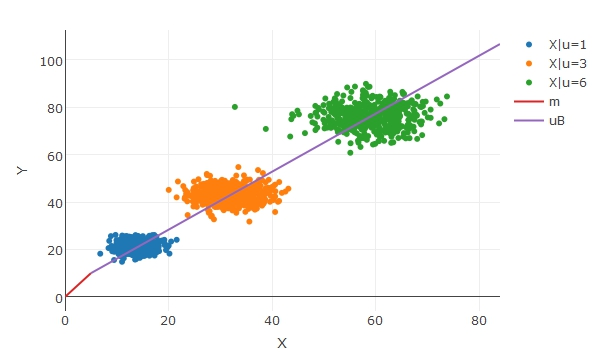
\includegraphics[width=0.7\linewidth]{bm}
\caption{Nuevamente se asumió que u se distribuyó exponencial tomando los valores 1, 3 y 6, mientras que m=(5,10), B=(9,11), y la matriz de varianza covarianza fue la misma que en los ejemplos anteriores.}
\end{figure}



En la distribución de $X$ podemos considerar a $\mu$ como un vector de posición, mientras que $u\beta$ es un vector de dirección o tendencia.


Una propiedad importante de las variables de mezcla, es que el comportamiento de la cola del vector aleatorio $X$ dependende del comportamiento de la cola de la variable de mezcla $u$, por lo que se podría seleccionar alguna $u$ arbitraria para que $X$ tenga colas pesadas.

Y además, como se verá posteriormente, la función generadora de momentos $M_{x}(t)$ del vector aleatorio X es proporcional a $M_{u}(t)$, la función generadora de momentos de la variable de mezcla u. Y la función característica $\Phi_{x}(it)$ es proporcinal a la función característica de la variable de mezcla u, $\Phi_{u}(it)$.\\





\pagebreak
\subsection*{Propiedades}

1) La función característica de $X$ es: 
\begin{equation*}
\Phi_{X}(t)=\exp(it\mu\acute{})\Phi_{u}(it\beta\acute{}-\frac{1}{2}t\Delta t\acute{}) 
\end{equation*}
Donde $\Phi_{u}(.)$ es la función característica del la variable de mezcla u. \\

Demostración:\\
\begin{equation*}
\Phi_{X}(t)=\underset{x}{\int }\exp(it)f(x)dx = \underset{x}{\int }\exp(it)(\underset{u}{\int}f(x)|_{u}f(u)du)dx=
\end{equation*}
\begin{equation*}
\underset{x}{\int}\underset{u}{\int}exp(it)f(x)|_{u}f(u)dudx
\end{equation*}


Luego por el Teorema de Fubini (ver algún anexo)\\
\begin{equation*}
\underset{x}{\int}\underset{u}{\int}exp(it)f(x)|_{u}f(u)dudx=\underset{u}{\int}\underset{x}{\int}exp(it)f(x)|_{u}f(u)dudx=
\end{equation*}
 \begin{equation*}
 \underset{u}{\int}exp(it(\mu+ u\beta)+\frac{1}{2}itu\Delta it)f(u)du
 \end{equation*}
  

Ya que la función generadora de momentos de una distribución normal p-variada es: $exp(t\acute{}\mu + t\acute{}\Sigma t)$, y además $X$ dado $u$ se distribuye $N(\mu + u\beta, u\Delta)$ \\

Factorizando el exponenete de la exponencial se tiene que:\\
\begin{equation*}
\underset{u}{\int}exp(it(\mu+ u\beta)+\frac{1}{2}itu\Delta it)f(u)du=
\end{equation*}
\begin{equation*}
\underset{u}{\int}\exp(it\acute{}\mu)exp(u(it\acute{}\beta -\dfrac{1}{2}t\acute{}u \Delta t))f(u)du = exp(it\acute{}\mu)\Phi_{u}(it\beta-\frac{1}{2}t\Delta t)
\end{equation*}
Por lo tanto: 
\begin{equation*}
\Phi_{X}(t) = exp(it\acute{}\mu)\Phi_{u}(it\beta-\frac{1}{2}t\Delta t)
\end{equation*}

Para comprobar que la función generadora de $X$ es:
\begin{equation*}
M_{x}(t)=\exp^{t\acute{}\mu}M_{u}(t\beta+\dfrac{1}{2}t\acute{}\Delta t)
\end{equation*}
  basta con sustituir $t$ por $it$ en el resultado anterior.\\

El resultado anterior nos indica que podemos obtener la función generadora de momentos o característica del vector aleatorio $X$ con tan solo conocer la función característica o generadora de la variable aleatoria $u$, lo cual sería de utilidad si solo nos interesan algunos momenots, o también nos ayudaría a identificar la distribución de $X$, en caso de reconocer la función característica o generadora de momentos. Inversamente, el resutado anterior también nos indica que si la función característica o generadora de algún vector aleatorio $Z$ se puede descomponer como el producto de $\exp{it\acute{}\mu} $, y alguna $M_{y}(t)$, entonces $Z$ es una variable normal de mezcla en esperanza-varianza, con distribución de mezcla $y$.\\

\chapter*{Inferencia estadística}
En este capítulo se verá lo que es una distribución tipo mezcla en general, así como algunas de sus utilidades, para después enfocarnos en la mezcla que nos es de interés, es decir, la mezcla continua. Luego se ahondará en cómo estimar los parámetros de las mezclas compuestas a través del método de máxima verosimilitud, y la necesidad de extender la verosimilitud. Por último, se propondrá seleccionar el muestreador de Gibbs para encontrar los parámetros de interés de nuestra mezcla.\\

\subsection*{Distribuciones tipo mezcla numerable}
Este tipo de distribución consiste en ponderarar un conjunto numerable de vectores aleatorios $X_{i}$  discretos con el mismo soporte y la misma dimención con un conjunto de pesos, positivos y menores a uno, $w_{i}$, donde $i$ proviene de un conjunto $I$ de índices numerable, y a su vez $\sum_{i\in I}w_{i}=1$. El índice $i$ puede ser generado por una distribución de probabilidad discreta, en este caso $P(i)=w_{i}$ por lo que a los pesos también se les conoce como probabilidades. Entonces la función de densidad es de la siguiente forma:\\
\begin{equation*}
f_{x}(x)= \sum_{i\in I}w_{i}f{X_{i}}(x)
\end{equation*}
 Donde  $0<w_{i}<1$, $\sum_{i\in I}w_{i}=1,$ y $  f_{X_{i}}(x)$ es un vector aleatorio discreto de dimención p para todo $i$ en $I$.\\

Es común encontrar este tipo de distribuciones en un conjunto de datos que provienen de dos o más distribuciones diferentes, lo cual podría resultar en una distribución multimodal. Si el conjunto de vectores aleatorios provienen de la misma distribución, entonces se dice que es una mezcla de familias paramétricas, mientras que si el vector aleatorio tienen una distribución continua, entonces se le conoce como densidad tipo mezcla continua.\\

\subsection*{Densidad tipo mezcla continua}
Una densidad tipo mezcla continua resulta de considerar que los pesos $w$ están dados por una densidad continua $f_{w}(w)$ con soporte en $R_{+}$, a $w$ se le conoce como variable de mezcla. Ahora, el vector aleatorio $X$ está parametrizado por $(\theta,w)$, por lo que ahora la familia de vectores aleatorios queda dada por la familia no numerable  $ X$ dado $w$, tal que $w$ se distribuye $f_{w}(w) $, de aquí que la densidad de $X$ esté dada por:\\
\begin{equation*}
f_{x}(x)=\int_{0}^{\infty}f(x|w)f_{w}(w)dw 
\end{equation*}


Si $w$ es una variable aleatoria con distribución paramétrica, es común que la distribución de $X$ dependa de los parámetros de $u$, y además ciertas características como la disperción o la cola de la distribución de $X$ también dependerán de las características de la variable de mezcla $w$.\\



\subsection*{Función de verosimilitud y verosimilitud extendida}

 De entre los distintos métodos de estimación de distribuciones paramétricas se usará el de máxima verosimilitud debido a las propiedades de estos estimadores, y a que actualmente existen métodos computacionales que permiten obtener dichos estimadores sin necesidad de que la distribución del vector aleatorio $X$ tenga una forma analítica.\\

Supongamos que tenemos una muestra aleatoria independiente e idénticamente distribuida de tamaño n del vector aleatorio $X\in R^{p}$, y que además, la distribución de $X$ puede ser estudiada a partir de una distribución tipo mezcla, con variable de mezcla $u$, entonces como los parámetros de $X$ dependerán de la variable de mezcla $u$, la propiedad de invarianza de los estimadores máximo verosimiles nos permite hacer la inferencia sobre los parámetros de la distribución de mezcla y la variable de mezcla, por lo que la función de verosimilitud está dada de la siguiente forma:\\

\begin{equation*}
P(X_{1}=x_{1},..., X_{n})=\prod_{i=1}^{n}P(X_{i}=x_{i})=\prod_{i=1}^{n} \underset{u}{\int } f(X_{i}=x_{i}|\theta,u)f_{u}(u|\alpha)du
\end{equation*}
Donde $\Theta$ son los parámetros correspondientes a la distribución de $X$ dado $u$, mientras que $\alpha$
son los parámetros de la distribución de mezcla $u$.
Ahora, suponiendo que se cumplen las condiciones de regularidad se tiene que:
\begin{equation*}
Lik(\theta,\alpha)= \underset{u}{\int }\prod_{i=1}^{n} f(X_{i}=x_{i}|\theta,u)f_{u}(u|\alpha)
\end{equation*}


La última expresión obtenida parece complicada a simple vista, pues además del producto de lasfunciones de densidad, hay un proceso de integración, lo cual nos lleva a buscar una alternativa para manejar la función de verosimilitud, lo cual se logra a través de extender la verosimilitud.

\subsection*{Verosimilitud extendida}

El proceso de extender la verosimilitud consiste en tratar al vector aleatorio $X$ p dimensional como una variable tipo mezcla, donde la variable de mezcla $u$ se considera como latente. Este método pretende encontrar los mejores estimadores para la variable tipo mezcla $u$, y a su vez que esta variable de la más verosimil probabilidad de haber observado al vector $X$.\\ 

\pagebreak
Por ejemplo, supongamos que $X$ es una variable aleatoria Pareto(1,$\beta$), de la cual tenemos  una realización $X_{0} $, y que nos interesa estimar el valor de $ \beta$, luego sea $X$ dado $u$ una distribución exponencial con parámetro $\lambda$, y además supóngase que $ \lambda$ también es una variable exponencial con parámetro $\beta $. Entonces, $X$ se puede expresar como una mezcla de distribuciones exponenciales como sigue:\\
\begin{equation*}
f_{X}(x)=\underset{0}{\overset{\infty }{\int }}f_{x|\lambda}(x)f_{\lambda}(\lambda)d\lambda=\underset{0}{\overset{\infty }{\int }} \lambda \exp^{-\lambda x} \beta \exp^{-\beta \lambda} d\lambda=\dfrac{\beta}{(x+\beta)^{2}}
\end{equation*}


Ahora, si consideramos la distribución de $ X$ dado $\lambda_{i}$, para cada $\lambda_{i}$ tendríamos una densidad diferente. En la siguiente figura se ilustra la densidad de $X$ dado $\lambda$, para algunos valores de $ \lambda$.\\

\begin{figure}[h]
\centering
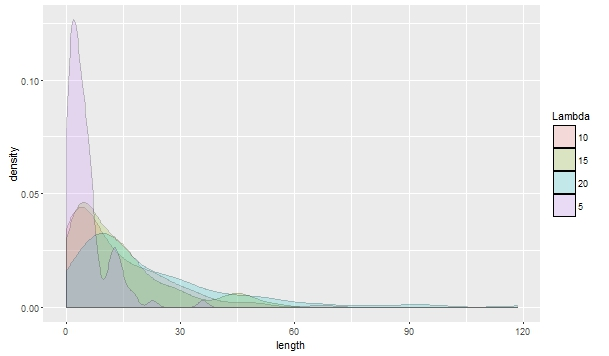
\includegraphics[width=0.7\linewidth]{LAMBDAS}
\caption{Se graficaron distribuciones exponenciales con parámetro $\lambda=5, 10, 15, 20$}
\end{figure}

De aquí, que nos podríamos plantear la siguiente pregunta ¿Dada una observación $ X_0$, cual sería la $ \lambda_{i}$ que le asigne mayor probabilidad o densidad a la ocurrencia de esta observación? Por ejemplo, de la gráfica anterior se puede observar que si $x_{0}=5$ , el mejor valor de lambda sería $\lambda=5$, mientras que si $x_{0}=30$, sería $\lambda=15$. En la misma línea, también sería acertado preguntarse por el mejor estimador de $\beta$, donde la probabilidad de que ocurra la $\lambda_{i}$ (que maximiza la la probabilidad de ocurrencia de $x_{0}$) sea máxima. Entonces, si consideramos la función de verosimilitud para $X_{0}$, sería:\\
\begin{equation*}
 Lik(\beta|X)=f_{x}(x)=\dfrac{\beta}{(x+\beta)^{2}}=\underset{0}{\overset{\infty }{\int }}f_{x|\lambda}(x)f(\lambda)d\lambda
\end{equation*}

 
Y con el planteamiento anterior, en lugar de buscar el mejor estimador de $\beta$ en Lik($\beta|X_{0}$), podríamos preguntarnos por la mejor $\lambda_{i}$ inducida por $\beta$ tal que $\beta$ maximice la ocurrencia de $\lambda_{i}$, y a su vez, $\lambda_{i}$ maximice la probabilidad de haber observado  $X_{0}$,  entonces con este enfoque, la función de verosimilitud para $X_{0}$ queda expresada de la siguiente manera:

\begin{equation*}
Lik(\lambda_{i},\beta|X_{0})=f_{x|\lambda_{i}}(x|\beta,\lambda_{i})f(\lambda{i})
\end{equation*}
	
	Siguiendo el plantemiento anterior, la verosimilitud extendida se define de la siguiente forma:\\
	
	Sean ${X}_{i=1}^{n}$ un conjunto de vectores aleatorios independientes e idénticamente distribuidos de dimención p con algún vector de parámetros $\theta$, y sea $u$ una variable aleatoria con algún vector de parámetros $\beta$ y con soporte en $R_{+}$, tal que $X_{i}$ se puede esxpresar como una distribución tipo mezcla con variable de mezcla $u$. Entonces  $f_{X_{i}}(x_{i})=\underset{0}{\overset{\infty }{\int }}f_{x_{i}|u}(x_{i})f_{u}(u)du$ para toda $i$, con $X_{i}$ dado $u_{i}$ condicionalmente independiente a $X_{j}$ dado $u_{j}$, y $ u_{i}$ dado $\beta$ independiente a $u_{j}$ dado $\beta$ para toda $i$ diferente de $j$, entonces:\\
	\begin{equation*}
	Lik(u_{i},\theta,\beta |X)=\prod_{i=1}^{n}f_{x_{i}|u_{i}}(x|\theta, u_{i},\beta)f_{u_{i}}(u_{i}|\beta)
	\end{equation*}
	
	
	donde $u_{i}$ es una variable latente.\\
	
	Trabajar con la verosimilitud extendida podría parecer más complicado al tener que estimar una variable latente para cada observación de $X$, pero en ocasiones resulta más sencillo optimizar la función $\prod_{i=1}^{p}f_{x_{i}|u_{i}}(x_{i})f(u_{i})$ que $f(X)$, y además, existen algoritmos computacionales, vía cadenas de Markov, o el algoritmo EM, que permiten encontrar los estimadores de los parámetros deseados. Por lo que ahora nuestro objetivo será seleccionar un algoritmo que nos permita trabajar con la verosimilitud extendida.



\subsection*{Muestreador de Gibbs}

El muestreador de Gibbs es un método de simulación, que permite obtener una muestra de una distribución conjunta a partir de las distribuciones marginales. Entre los principales usos de este algoritmo, es obtener una muestra de los parámetros de interés de algún modelo probilístico, a partir de las distribuciones condicionadas de los parámetros. Este método consiste en construir una cadena de Markov, para así conseguir una muestra de una distribución dada, la construcción de la cadena de Markov es necesaria para asegurar que nuestrra muestra proviene efectivamente de la distribución que nos interesaría muestrear. Por lo que en la siguiente parte se verá el planteamiento y la forma de implementar este algoritmo para obtener una muestra de parámetros de interés. \\

Supongamos que tenemos una distribución de la forma $f(X,\Theta)$ donde X es un vector aleatorio y $\Theta$ algún vector de parámetors del cual se desearía tener una muestra mediante una cadena de Markov, es decir, obtener una muestra de $f(\theta ^{k}|X)$ a partir de una sucesión de parámetros ${\theta}_{1} ^{\infty}$, tal que la probabilidad de transición de esta sucesión converga a la distribución de la cual se desearía tener una muestra, esto es, $\lim_{k->\infty} P(\theta^{k+1}|\theta^{k},X)=P(\theta|X)$. Dada la descripción del modelo anterior, la cadena debe ser: estacionaria, irreducible, aperiódica y recurrente positiva. La propiedad de estacionariedad asegurar que $P(\theta|X)$ no cambie cuando $k$ tienda a infinito, irreducible para no descartar ningún valor posible de $\theta ^{k}$ en cada iteración, mientras que aperiodicidad para que la cadena no tenga ciclos, y así permanecer en el estado estacionario. Por último, recurrente positiva, para que se pueda visitar cualquier estado un número infinito de veces para así asegurar que la distribución límite tomó toda la información disponible en consieración.\\

Ahora bien, para encontrar una cadena que nos permita obtener las caractrísticas anteriores German $\&$ German (citar bien esta parte) demuestra que  $ \lim_{k->\infty} P(\theta^{k}|X)=P(\theta|X)$, donde:
\begin{equation*}
 P(\theta^{k}|X)=\stackrel{~}{{\prod}_{j=1}^{t }}P(\theta_{j}|X,...,\theta_{j-1},\theta_{j+1},...,\theta_{n}) 
\end{equation*}

 donde $\theta_{j}$ dado $X,...,\theta_{j-1},\theta_{j+1},...,\theta_{n}$ es condicionalmente independiente para toda $j$, para alguna medida de probabilidad arbitraria $P(.)$. Entonces si $\theta_{j} ^{k}$ se distribulle $ f(\theta_{j} ^{k}|X,...,\theta_{j-1},\theta_{j+1},...,\theta_{n})$, de aquí sería fácil obtener una muestra de $\theta_{j} ^{k}$ para toda $j$, si su densidad tiene una forma cerrada, y así se construiría una cadena de markov con las caractarísticas deseadas, $[\theta^{k}] _{1} ^{\infty}$, con probabilidad de transición $P(\theta^{k}|X)$.\\

Entonces los pasos para implementar el Muestreador de Gibbs son los siguientes:\\

Dar un conjunto de valores iniciales $\Theta_{0}$, no importa que valores se den, la propiedad de estacionareidad, asegurará la convergencia al estado estacionario. El vector $\theta$ puede ser particionado en d subconjuntos excluyentes, tal que d$<=$n, con la finalidad de simplificar los cálculos. Estratégicamente se pueden seleccionar los sobconjuntos de modo que los que tienen alta correlación queden juntos.\\

Para cada $\theta_{j}$ obtener su distribución condicionada  $f(\theta_{j} |X,...,\theta_{0,j-1},\theta_{0,j+1},...,\theta_{0,n})$, y realizar una simulación de esta. El valor de $\theta_{j}$ obtenido reemplazará a los valores iniciales. En caso de que no se pueda tener la distribución de $\theta|_{X,\theta \ \theta_{j}}$ se realiza un procedimiento de aceptación rechazo para obtener una realización de $\theta_{j}$.\\

Una vez obtenidos todos los valores de $\theta|_{X,\theta \ \theta_{j}}$ se reemplazan por los valores iniciales y se repite el procedimiento hasta que la cadena se estabilice.

computacionalmente el algoritmo se vería de la siguiente forma:\\
\begin{center}
	$\Theta_{k} <- (\theta_{1,0},...,\theta_{d,0})$\\
	do{while $||\theta^{k+1}-varaux< \epsilon || $ }\\
		$varaux<-\theta_{k}	$\\
		for (j in 1:d)c\\
			$\theta_{j} ^{k+1}<-$ random (f($\theta|_{X,\theta^{k} \ \theta_{j} ^{k}}$))\\
		              
	end do while\\
\end{center}
									

\section*{Inferencia de los parámetros de una distribución Hiperbólica generalizada}

Supongamos que tenemos una colección de $r_{n}$ datos, donde cada $r_{i}\in R^{p}$, de los cuales tenemos motivos para creer que fueron generados por una distribución hiperbólica generalizada p-variada. Entonces nos interesaría inferir los valores de los parámetros de dicha distribución, pero antes de ello sería conveniente expreasar a nuestra distribución de interés como una distribución tipo mezcla normal, con variable de mezcla $u$ distribuidad gaussiana inversa generalizada (GIG), por lo que así podemos replantear el problema, enfocandonos en buscar los parámetros de la distribución de mezcla, $\mu,\beta,\Sigma$.\\

Ahora sobre un enfoque bayesiano, podemos plantear la verosimilitud de la distribución aposteriori de $\mu,\beta,\Sigma$, es decir:
\begin{equation*}
f(\mu,\beta,\Sigma|(r_{i})_{i=1}^{n})=\prod_{i=1}^{n}f_{r_{i}}(r_{i}|\mu,\beta,\Sigma)\Pi(\mu,\beta,\Sigma)
\end{equation*}   
Donde $\Pi(\mu,\beta,\Sigma)$ es la distribución conjunta a priori de $\mu,\beta$ y $\Sigma$, y además asumiremos que tanto $\mu,\beta,\Sigma$ son independientes, por lo que:
\begin{equation*}
f(\mu,\beta,\Sigma|(r_{i})_{i=1}^{n})=\prod_{i=1}^{n}f_{r_{i}}(r_{i}|\mu,\beta,\Sigma)\Pi(\mu|\mu_{0},\Sigma_{0})\Pi(\beta|\mu_{\beta},\Sigma_{\beta})\Pi(\Sigma|S)
\end{equation*}
 Como supuesto adicional, asumiremos que $\mu$ se distribuye $N(\mu_{0},\Sigma_{0})$, $\beta$ se distribuye $N(\beta_{0},\Sigma_{\beta})$, y $\Sigma$ se distribuye $W(S)$. Por lo que nuestra función de verosimilitud adquiere la siguiente forma:
\begin{equation*}
Lik(\mu,\mu_{0},\beta,\beta_{0},\Sigma,\Sigma_{0},\Sigma_{\beta},S|(r_{i})_{i=1}^{n})=
\end{equation*}
\begin{equation*}
\prod_{i=1}^{n}\int_{0}^{\infty}N_{p}(r_{i}|\mu,u\beta,u\Sigma)GIG(u|\lambda_{0},\xi_{0},\Psi_{0})du N_{p}(\mu|\mu_{0},\Sigma_{0})N_{p}(\beta|\beta_{0},\Sigma_{\beta})W_{pxp}(\Sigma|S)
\end{equation*}

Ahora según lo expuesto en el capítulo 3.algo, es conveniente extender la verosimilitud, por lo que ahora tenemos que:
\begin{equation*}
Lik(\mu,\mu_{0},\beta,\beta_{0},\Sigma,\Sigma_{0},S,(u_{i})_{i=1}^{n}|(r_{i})_{i=1}^{n})=
\end{equation*}
\begin{equation*}
\prod_{i=1}^{n}N_{p}(r_{i}|\mu,u_{i}\beta,u_{i}\Sigma)GIG(u_{i}|\lambda_{0},\xi_{0},\Psi_{0})du N_{p}(\mu|\mu_{0},\Sigma_{0})N_{p}(\beta|\mu_{\beta},\Sigma_{\beta})W_{pxp}(\Sigma|S)
\end{equation*}

Una vez teniendo nuestra función de verosimilitud, ya estamos en condiciones de proponer algún método númerico para encontrar los parámetros de interés; ya que se ha empleado el enfoque bayesiano, y por la forma de las distribuciones tipo mezcla es conveniente implementar el muestreador de Gibbs.\\

Por lo que ahora necesitamos conocer las distribuciones marginales de 
$\mu|\beta,\Sigma,(u_{i})_{i=1}^{n},(r_{i})_{i=1}^{n}$, $\beta|\mu,\Sigma,(u_{i})_{i=1}^{n},(r_{i})_{i=1}^{n}$, $\Sigma|\mu,\beta,(u_{i})_{i=1}^{n},(r_{i})_{i=1}^{n}$, y $u_{j}|\beta,\Sigma,(u_{i\ne  j})_{i=1}^{n},(r_{i})_{i=1}^{n} \forall j$, lo cual se mostrará en la siguiente parte.

\subsection*{Distribución marginal de $\mu$}
Para en contrar la distribución marginal de $\mu|\beta,\Sigma,(u_{i})_{i=1}^{n},(r_{i})_{i=1}^{n}$, a partir de la función de verosimilitud podemos tomar las densidades donde aparece $\mu$ e identificar su kernel, es decir, de: 
\begin{equation*}
\prod_{i=0}^{n}N_{p}(r_{i}|\mu,u_{i}\beta,u_{i}\Sigma)N_{p}(\mu|\mu_{0},\Sigma_{0})=
\end{equation*}
\begin{equation*}
\prod_{i=1}^{n}\dfrac{exp(-\frac{1}{2}(r_{i}-\mu-u_{i}\beta)'(u_{i}\Sigma)^{-1}(r_{i}-\mu-u_{i}\beta))}{(2u_{i}\Pi)^{p/2}|\Sigma|^{1/2}}\dfrac{exp(-\frac{1}{2}(\mu-\mu_{0})'\Sigma_{0}(\mu-\mu_{0}))}{(2\Pi)^{p/2}|\Sigma|^{1/2}}
\end{equation*}
tomando el cambio de variable  $r_{i}\acute{}=r_{i}-u_{i}\beta$, nos quedamos con 
\begin{equation*}
\prod_{i=1}^{n}exp(-\frac{1}{2}(\mu-r_{i}')'(u_{i}\Sigma)^{-1}(\mu-r_{i}'))exp(-\dfrac{1}{2}(\mu-\mu_{0})'\Sigma_{0}(\mu-\mu_{0}))
\end{equation*}
Después, trabajando únicamente con
\begin{equation*}
\prod_{i=1}^{n}exp(-\frac{1}{2}(\mu-r_{i}')'(u_{i}\Sigma)^{-1}(\mu-r_{i}'))=exp(-\frac{1}{2}\sum_{i=1}^{n}(\mu-r_{i}')'(u_{i}\Sigma)^{-1}(\mu-r_{i}'))
\end{equation*}
\begin{equation*}
exp(-\frac{1}{2}\sum_{i=1}^{n}(\mu'(u_{i}\Sigma)^{-1}\mu  -2\mu(u_{i}\Sigma)^{-1}r_{i}' -r_{i}'(u_{i}\Sigma)^{-1}r_{i}' )\alpha 
\end{equation*}
\begin{equation*}
\alpha exp(-\frac{1}{2}\sum_{i=1}^{n}(\mu'(u_{i}\Sigma)^{-1}\mu  -2\mu(u_{i}\Sigma)^{-1}r_{i}')=
\alpha exp(-\frac{1}{2}(\mu'(U\Sigma)^{-1}\mu  -2\mu(U\Sigma)^{-1}R)
\end{equation*}
Donde : 
\begin{equation*}
U=(\sum_{i=1}^{n}\dfrac{1}{u_{i}})^{-1}, R= \sum_{i=1}^{n}\dfrac{r_{i}}{u_{i}}U
\end{equation*}
Entonces, según el anexo 4 esta parte del kernel de $\mu$ le corresponda una distribución normal p variada con vector de medias $R$, y matriz de varianza covarianza $U\Sigma$. Luego, multiplicando el kernel anterior por la densidad de $\mu$, y por el anexo 6 se tiene que $\mu$ se distribuye normal con vector de medias:
\begin{equation*}
(R(U\Sigma)^{-1}+\mu_{0}\Sigma_{0}^{-1})(U\Sigma^{-1}+\Sigma_{0}^{-1})^{-1}
\end{equation*}
 y matriz de varianza covarianza:
 \begin{equation*}
 U\Sigma+\Sigma_{0}
 \end{equation*}

\subsection*{Distribución marginal de $\beta$}
Ahora mediante un procedimiento similar a lo descrito anteriormente, encontraremos el Kernel de $\beta$ dado las demás variables de interés. Entonces, de la función de verosimilitud, nos quedamos con la parte donde sólo aparece $\beta$, es decir:
\begin{equation*}
\prod_{i=0}^{n}N_{p}(r_{i}|\mu,u_{i}\beta,u_{i}\Sigma)N_{p}(\beta|\mu_{\beta},\Sigma_{\beta})
\end{equation*}
Luego trabajando con el producto de las n variables normales p variadas correspondientes a $r_{i}$,  considerando los términos que únicamente dependen de $\beta$, y con el cambio de variable $\mu_{i}=r_{i}-\beta$, tenemos que:
\begin{equation*}
\prod_{i=1}^{n}exp(-\dfrac{1}{2}(r_{i}-\mu-u_{i}\beta)'(u_{i}\Sigma)^{-1}(r_{i}-\mu-u_{i}\beta))=
\end{equation*}
\begin{equation*}
exp(-\frac{1}{2}\sum_{i=1}^{n}((u_{i}\beta-\mu_{i})'(u_{i}\Sigma)^{-1}(u_{i}\beta-\mu_{i}))
\end{equation*}

Nuevamente desarrollando el exponente de la función exponencial, y quedandonos únicamente con la parte que depende de $\beta$ tenemos que:
\begin{equation*}
exp(-\dfrac{1}{2}\sum_{i=1}^{n}((u_{i}\beta)'(u_{i}\Sigma)^{-1}(u_{i}\beta)-2(u_{i}\beta)'(u_{i}\Sigma)^{-1}\mu_{i}))=
\end{equation*}
\begin{equation*}
exp(-\dfrac{1}{2}(\beta(V\Sigma)^{-1}\beta-2\beta(V\Sigma)^{-1}VM)
\end{equation*}
Donde:
\begin{equation*}
V=\frac{1}{\sum_{i=1}^{n}u_{i}} , M=\sum_{i=1}^{n}(r_{i}-\mu)
\end{equation*}
 Por lo tanto, según el anexo 4, el Kernel del producto de las n variables normales p variadas correspondientes a $\beta$ corresponde a una distribución normal con vector de medias $VM$, y matriz de varianza covarianza $V\Sigma$.
Luego, según el anexo 6, juntando el kernel obtenido anteriormente con la densidad de $\beta$, se tiene que $\beta$ se distribuye normal p variado con vector de medias: 
\begin{equation*}
(MV\Sigma)^{-1}+\mu_{\beta}'\Sigma_{\beta}^{-1})((V\Sigma)^{-1}+\Sigma_{\beta}^{-1})^{-1}
\end{equation*}
Y matriz de varianza covarianza:
\begin{equation*}
V\Sigma+\Sigma_{\beta}
\end{equation*}

\pagebreak

\section*{Distribución Gaussiana inversa generalizada}
Se dice que $X$ tiene una distribución gaussiana inversa generalizada $N\tilde{}(\lambda,\xi,\Psi)$, si su densidad es de la siguiente forma:

\begin{equation*}
f(x)= \dfrac{\xi^{-\lambda}\sqrt{\xi\Psi}^{\lambda}x^{\lambda-1}\exp{\frac{-1}{2}(\xi x^{-1} + \Psi x)}}{2\kappa_{\lambda}(\sqrt{\xi\Psi})}  
\end{equation*}

Donde $\kappa_{\lambda(.)}$ es una función modificada de Bessel de tercer tipo, y si $\lambda<0$, entonces $\xi>0$, $\Psi \ge 0 $; y si $\lambda=0$, entonces $\xi>0$, $\Psi > 0 $, y si si $\lambda>0$, entonces $\xi\ge 0$, $\Psi > 0 $.\\

Si $X$ se distribuye $N\tilde{}(\lambda,\xi,\Phi)$, entonces su función generadora de momentos es:
\begin{equation*}
\Phi (it)=\underset{-\infty }{\overset{\infty }{\int }}\exp{itx}\dfrac{\xi^{-\lambda}\sqrt{\xi\Psi}^{\lambda}x^{\lambda-1}\exp{\frac{-1}{2}(\xi x^{-1} + \Psi x)}}{2\kappa_{\lambda}(\sqrt{\xi\Psi})}dx=
\end{equation*}
\begin{equation*}
\frac{\sqrt{\xi\Psi}^{\lambda}}{2\kappa_{\lambda}(\sqrt{\xi\Psi})}\frac{2\kappa_{\lambda}(\sqrt{\xi(2it + \Psi)})}{\sqrt{\xi(2it + \Psi)}^{\lambda}}\underset{-\infty }{\overset{\infty }{\int }}\xi^{-\lambda}\frac{\sqrt{\xi(2it + \Psi)}^{\lambda}}{2\kappa_{\lambda}(\sqrt{\xi(2it + \Psi)})}\exp{\frac{-1}{2}(\xi x^{-1} + (2it+\Psi) x)}
\end{equation*}
Donde la última integral vale uno por ser una densidad $N\bar{}(\lambda,\xi,2it + \psi)$ integrada sobre su soporte, por lo que:

\begin{equation*}
\Phi(it)=\frac{\sqrt{\xi\Psi}^{\lambda}}{\kappa_{\lambda}(\sqrt{\xi\Psi})}\frac{\kappa_{\lambda}(\sqrt{\xi(2it + \Psi)})}{\sqrt{\xi(2it + \Psi)}^{\lambda}}
\end{equation*}

Si $X$ se distribuye $N\tilde{}(\lambda,\xi,\Phi)$, entonces su r-ésimo momento es:
\begin{equation*}
E[X^{r}]=\underset{-\infty }{\overset{\infty }{\int }}x^{r}\dfrac{\xi^{-\lambda}\sqrt{\xi\Psi}^{\lambda}x^{\lambda-1}\exp{\frac{-1}{2}(\xi x^{-1} + \Psi x)}}{2\kappa_{\lambda}(\sqrt{\xi\Psi})}dx=
\end{equation*}
\begin{equation*}
\frac{x^{r}2\kappa_{\lambda+r}(\sqrt{\xi\Psi})}{\sqrt{\xi\Psi}^{r}2\kappa_{\lambda}(\sqrt{\xi\Psi})}\underset{-\infty }{\overset{\infty }{\int }}\dfrac{\xi^{-\lambda-r}\sqrt{\xi\Psi}^{\lambda+r}x^{\lambda+r-1}\exp{\frac{-1}{2}(\xi x^{-1} + \Psi x)}}{2\kappa_{\lambda+r}(\sqrt{\xi\Psi})}dx
\end{equation*}
Por lo tanto:
\begin{equation*}
E[X^{r}]=(\frac{\xi}{\Psi})^{\frac{r}{2}}\frac{\kappa_{\lambda+r}(\sqrt{\xi \Psi})}{\sqrt{\kappa_{\lambda}(\sqrt{\xi\Psi})}}
\end{equation*}
\section*{Distribución Hiperbólica Generalizada}
Se dice que el vector p variado $X$ tiene una distribución hiperbólica generalizada $GH_{p}(\lambda,\xi,\Psi,\mu,\Sigma,\beta)$ si su densidad es de la siguiente forma:
\begin{equation*}
f(x)=c\frac{\kappa_{\lambda-d/2}(\sqrt{\xi +(x-\mu)'\Sigma^{-1}(x-\mu)(\Psi+\beta\acute{}\Sigma^{-1}\beta)})}{\xi + (x-\mu)'\Sigma^{-1}(x-\mu)(\Psi+\beta'\Sigma^{-1}\beta)^{\frac{d}{2}-\lambda}}\exp{(x-\mu)'\Sigma^{-1}\beta}
\end{equation*}

donde c=$\frac{\sqrt{\xi\lambda}^{-\lambda}\Psi^{\lambda}(\Psi+\beta\acute{} \Sigma^{-1}\beta)^{\frac{d}{2}-\lambda}}{(2\Pi)^{\frac{d}{2}}|\Sigma|^{\frac{1}{2}}\kappa_{\lambda(\sqrt{\xi\Psi})}}$. \\


Una característica importante de la distribución hiperbólica generalizada es que puede descomponerse como una variable de mezcla, donde $X|u$ se distribuye $N(\mu+u\beta,u\Sigma)$, y u se distribuye $N\bar{}(\lambda,\xi,\Psi)$.

\begin{equation*}
f(x)=\underset{-\infty }{\overset{\infty }{\int }}\frac{\exp{(x-\mu)'\Sigma^{-1}(x-\mu)}}{(2\Pi)^{d/2}|\Sigma|^{1/2}u^{d/2}}\exp{-\dfrac{(x-\mu)'\Sigma^{-1}(x-\mu)}{2u}}-\frac{\beta\Sigma^{-1}\beta}{2/u}f(u)du
\end{equation*}
Donde:
\begin{equation*}
f(u)=\dfrac{\xi^{-\lambda}\sqrt{\xi\Psi}^{\lambda}u^{\lambda-1}\exp{\frac{-1}{2}(\xi u^{-1} + \Psi u)}}{2\kappa_{\lambda}(\sqrt{\xi\Psi})} 
\end{equation*}

Sea $a=(x-\mu)'\Sigma^{-1}(x-\mu)$, y $b=\beta\Sigma^{-1}\beta$, entonces de aquí se sigue que:

\begin{equation*}
f(x)=\frac{\exp{(x-\mu)'\Sigma^{-1}\beta}\xi^{-\lambda}\sqrt{\xi\Psi}^{\lambda}}{(2\Pi)^{d/2}|\Sigma|^{1/2}2k_{\lambda}(\sqrt{\xi\Psi})}\underset{-\infty }{\overset{\infty }{\int }}u^{\lambda - d/2 -1}\exp{-1/2(au^{-1}bu+\xi u^{-1}+\Psi u)}du
\end{equation*}
Trabajando solamente con el integrando se tiene que:
\begin{equation*}
\underset{-\infty }{\overset{\infty }{\int }}u^{\lambda - d/2 -1}\exp{-1/2(au^{-1}+bu+\xi u^{-1}+\Psi u)}du=
\end{equation*}
\begin{equation*}
\underset{-\infty }{\overset{\infty }{\int }}u^{\lambda -d/2 -1}\exp{-1/2((a+\xi)u^{-1}+(b+\Psi)u} du
\end{equation*}
Ahora, sea $\lambda\acute{}=\lambda- 1/2$, $\xi\acute{}=a+\xi$, $\Psi\acute{}=b+\Psi$, entonces:

\begin{equation*}
\underset{-\infty }{\overset{\infty }{\int }}u^{\lambda -d/2 -1}\exp{-1/2((a+\xi)u^{-1}+(b+\Psi)u} du=\underset{-\infty }{\overset{\infty }{\int }}u^{\lambda'-1}\exp{-1/2(\xi' u^{-1}+ \Psi'u)} du
\end{equation*}
Luego,
\begin{equation*}
\underset{-\infty }{\overset{\infty }{\int }}u^{\lambda'-1}\exp{-1/2(\xi' u^{-1}+ \Psi'u)} du=     \frac{2k_{\lambda'}(\sqrt{\xi'\Psi'})}{\xi'^{-\lambda'}(\sqrt{\xi'\Psi'})^{\lambda'}}   \underset{-\infty }{\overset{\infty }{\int }}\frac{\xi^{-\lambda'}(\sqrt{\xi\Psi})^{\lambda'}}{2k_{\lambda'}(\sqrt{\xi'\Psi'})}
\end{equation*}
\begin{equation*}
u^{\lambda'-1}\exp{-1/2(\xi' u^{-1}+ \Psi'u)} du
\end{equation*}

Donde la última integral vale uno por ser una distribución $N\bar{}(\lambda\acute{},\xi\acute{},\Psi\acute{})$ integrada sobre su soporte, por lo que tenemos que:\\

\begin{equation*}
f(x)=\frac{\exp{(x-\mu)'\Sigma^{-1}\beta}\xi^{-\lambda}\sqrt{\xi\Psi}^{\lambda}}{(2\Pi)^{d/2}|\Sigma|^{1/2}2k_{\lambda}(\sqrt{\xi\Psi})}\frac{2k_{\lambda'}(\sqrt{\xi'\Psi'})}{\xi^{-\lambda'}(\sqrt{\xi'\Psi'})^{\lambda'}}
\end{equation*}\\

Por último, sustituyendo los valores de $a$, $b$, $\xi\acute{}$, $\Psi\acute{}$, y agrupando algunos términos tenemos que efectivamente f(x) se distribuye $GH_{p}(\lambda,\xi,\Psi,\mu,\Sigma,\beta)$.\\

Ahora para encontrar los momentos de la distribución $GH_{p}$, como puede ser expresada como una variable de mezcla en esparanza-varianza, la propiedad 1) nos dice que $\Phi_{X}(t)=\exp(it\beta\mu\acute{})\Phi_{u}(it\beta\acute{}-\frac{1}{2}t\Sigma t\acute{})$, donde $\Phi_{u}(.)$ es la función característica del la variable de mezcla u que se distribuye $N\bar{}(\lambda,\xi,\Psi)$.\\

 La función característica nos permite calcular fácilmente la distribución de una transformación lineal del vector p-variado $X$, pues si ahora consideramos el vector aleatorio $Y=aX+b$, donde $a\in M_{rxp}$, $b\in R^{p}$ entonces:
\begin{equation*}
\Phi_{Y}(t)=exp(bit)\Phi_{X}(at)=\exp(bit+it\beta\mu\acute{})\Phi_{u}(iat\beta\acute{}-\frac{1}{2}at\Sigma at\acute{})=
\end{equation*}
\begin{equation*}
\exp(it(b+\beta\mu)\acute{})\Phi_{u}(iat\beta\acute{}-\frac{1}{2}at\Sigma at\acute{})
\end{equation*}
Lo cual nos indica que $Y$ se distribuye $GH_{p}(\lambda,\xi,\Psi,b+\beta\mu,a\Sigma a\acute{},a\beta)$, y a su vez que.\\

También a partir de la función característica es fácil ver que la distribución marginal de $X_{i}$ es 
$GH_{p}(\lambda,\xi,\Psi,\mu_{i},\Sigma _{i},\beta_{i})$, donde $\Sigma_{i}$ es el i-ésimo componente del primer renglón de $\Sigma$. Las dos propiedades anteriores nos dicen que si X se distribuye $GH_{p}$, entonces es cerrado bajo convoluciones.


\chapter*{Anexos}
\section*{Distribución normal p variada}
Se dice que el vector aleatorio $X\in R^{p}$ tiene una distribución normal p-variada $N_{p}(X|\mu,\Sigma)$ si su densidad es de la siguiente forma:
\begin{equation*}
f(X|\mu,\Sigma)=\dfrac{1}{(2\Pi)^{p/2}|\Sigma|^{1/2}}exp(-1/2(X-\mu)'\Sigma^{-1}(X-\mu))
\end{equation*}

Donde $\mu\in R^{p}$ es elvector de medias, y $\Sigma\in M_{pxp}$ es la matriz de varianza-covarianza.

\section*{Distribución tipo mezla normal p variada}
Se dice que el vector aleatorio $X\in R^{p}$ con densidad f(x) puede ser expresado como una distribución de mezcla normal $N(X|\mu,\beta,\Sigma)$ con variable de mezcla $u$ con densidad $f(u)$ y soporte en $R^{+}$, si:
\begin{equation*}
f(X|\mu,\beta,\Sigma)=\underset{0}{\overset{\infty }{\int }}N_{p}(X|\mu,u\beta,u\Sigma)f_{u}(u)du 
\end{equation*}

Donde, $N_{p}(X|\mu,u\beta,u\Sigma)$ es una distribución normal p-variada con vector de medias $\mu+u\beta$, y matriz de varianza-covarianza $u\Sigma$

\section*{Kernel de una distribución normal p variada}
El kernel un vector aleatorio es la parte de la función de densidad que únicamente depende de dicho vector, y a su vez nos permite identificar de que familia proviene la distribución. Por ejemplo, en el caso de la distribución normal p variada
\begin{equation*}
f(X|\mu,\Sigma)=\dfrac{1}{(2\Pi)^{p/2}|\Sigma|^{1/2}}exp(-\dfrac{1}{2}(x'\Sigma^{-1}x - x'\Sigma^{-1}\mu -\mu'\Sigma^{-1}x+\mu'\Sigma^{-1}\mu))
\end{equation*}
Tenemos que el Kernel correspondiente es:
\begin{equation*}
exp(-\dfrac{1}{2}(x'\Sigma^{-1}x -2x'\Sigma^{-1}\mu))
\end{equation*}
donde $\mu'\Sigma^{-1}x=x'\Sigma^{-1}\mu$, ya que es una forma cuadrática.
\section*{Kernel del producto de n distribuciones normales p variadas con mismo vector de medias y misma matriz de varianza covarianza}
Supongamos que $X_{i}$ se distribuye normal p variada con vector de media $\mu$ y matriz de varianza covarianza $\Sigma$, entonces la función de  interés es de la siguiente manera:
\begin{equation*}
\prod_{i=1}^{n}N(X_{i}|\mu,\Sigma)=\prod_{i=1}^{n}\dfrac{1}{(2\Pi)^{p/2}|\Sigma|^{1/2}}exp(-\frac{1}{2}(X_{i}-\mu)'\Sigma^{-1}(X_{i}-\mu))
\end{equation*}
De aquí, trabajando únicamente con el exponente de la función exponencial tenemos que:
\begin{equation*}
\prod_{i=1}^{n}exp(-\frac{1}{2}(X_{i}-\mu)'\Sigma^{-1}(X_{i}-\mu))=exp(-\frac{1}{2}\sum_{i=1}^{n} (X_{i}-\mu)'\Sigma^{-1}(X_{i}-\mu))=
\end{equation*} 
\begin{equation*}
exp(-\dfrac{1}{2}\sum_{i=1}^{n}(X_{i}'\Sigma^{-1}X_{i}-2X_{i}'\Sigma^{-1}\mu+\mu'\Sigma^{-1}\mu))=exp(-\frac{1}{2}(X'\Sigma^{-1}X-2X'\Sigma^{-1}\mu+n\mu\Sigma^{-1}\mu))
\end{equation*}
Donde la jésima coordenada del vector X es $\sum_{i=1}^{n}X_{i,j}$
Por último,como sólo nos interesan los términos donde aparece $X_{i}$, llegamos a que el kernel es:
\begin{equation*}
exp(-\frac{1}{2}(X'\Sigma^{-1}X-2X'\Sigma^{-1}\mu))
\end{equation*} 
\section*{Kernel del vector de medias de una distribución normal p variada multiplicada por la distribución del vector de medias}
En este caso tenemos que $X$ se ditribuye normal con vector de medias $\mu$ y matriz de varianza covarianza $\Sigma$, mientras que $\mu$ se distribuye normal con vector de medias $\mu_{0}$ y matriz de varianza covarianza $\Sigma_{0}$, y ahora nos interesa conocer el Kernel correspondiente a $\mu$, entonces tendríamos
que el producto de las funciones de densidad es:
\begin{equation*}
f_{X}(X|\mu,\Sigma)f_{\mu}(\mu|\mu_{0},\Sigma_{0})=    
\end{equation*}
\begin{equation*}
\dfrac{exp(-1/2(X-\mu)'\Sigma^{-1}(X-\mu))}{(2\Pi)^{p/2}|\Sigma|^{1/2}}       \dfrac{exp(-1/2(\mu-\mu_{0})'\Sigma_{0}^{-1}(\mu-\mu_{0}))}{(2\Pi)^{p/2}|\Sigma_{0}|^{1/2}}
\end{equation*}

Luego de cada función de densidad tomamos lo que dependa de $\mu$, para así obtener sus respectivos kerneles según el anexo 4,lo cual implica que:
\begin{equation*}
Kernel=exp(-\dfrac{1}{2}(\mu'\Sigma^{-1}\mu -2x'\Sigma^{-1}\mu))exp(-\dfrac{1}{2}(\mu'\Sigma_{0}^{-1}\mu -2\mu_{0}'\Sigma_{0}^{-1}\mu))=
\end{equation*} 
\begin{equation*}
exp(-\dfrac{1}{2}(\mu'\Sigma^{-1}\mu -2x'\Sigma^{-1}\mu + \mu'\Sigma_{0}^{-1}\mu -2\mu_{0}'\Sigma_{0}^{-1}\mu))=
\end{equation*}
\begin{equation*}
exp(-\frac{1}{2}(\mu'(\Sigma^{-1}+\Sigma_{0}^{-1})\mu-2(X'\Sigma^{-1}+\mu_{0}'\Sigma_{0}^{-1})\mu)=
\end{equation*}
\begin{equation*}
exp(-\frac{1}{2}(\mu'(\Sigma^{-1}+\Sigma_{0}^{-1})\mu-2(X'\Sigma^{-1}+\mu_{0}'\Sigma_{0}^{-1})(\Sigma^{-1}+\Sigma_{0}^{-1})^{-1}(\Sigma^{-1}+\Sigma_{0}^{-1})\mu))
\end{equation*}
De aquí se tiene que $\mu$ se distribuye normal p variada con matriz de varianza covarianza $\Sigma + \Sigma_{0}$, y vector de medias $(X'\Sigma^{-1}+\mu_{0}'\Sigma_{0}^{-1})(\Sigma^{-1}+\Sigma_{0}^{-1})^{-1}$


%----------------------------------------------------------------------------------------
%   APÉNDICE\beta
%----------------------------------------------------------------------------------------

\addtocontents{toc}{\vspace{2em}} % Agrega espacios en la toc

\appendix % Los siguientes capítulos son apéndices

%  Incluye los apéndices en el folder de apéndices

\include{Apendices/Ap}
\thispagestyle{empty}
%\include{Apendices/AppendixB}
%\include{Apendices/AppendixC}

\addtocontents{toc}{\vspace{2em}} % Agrega espacio en la toc


%----------------------------------------------------------------------------------------
%   BIBLIOGRAFÍA
%----------------------------------------------------------------------------------------
\backmatter
\nocite{*}
\bibliographystyle{plain}
\bibliography{bibliografía.bib} %Aquí ponen el nombre del archivo .bib






\end{document}
              
            


